\appendix
\section{chktex}
\begin{tiny}
\begin{verbatim}
cd ../../hid-sample; git pull
Already up to date.
cp ../../hid-sample/paper/Makefile .
cp ../../hid-sample/paper/report.tex .
WRNING: line longer than 80 characters
       212: \TODO{Decide whether to use six pis or 5 pis and the screen. If the former, the hardware description below will need to change. We could use the sixth pi in the other cluster we made and create a cluster of 11.}

WRNING: line longer than 80 characters
       92:   \centering\includegraphics[width=\columnwidth]{images/raspberry_pi_circuit_note_fig2.png}

WRNING: line longer than 80 characters
       206:   \caption{Pinout diagram of Raspberry Pi 3B~\cite{hid-sp18-419-pi-pinout}. Note: the Pi used for this project has a Broadcom BCM2837, not the Broadcom BMC2835 shown in this figure.}\label{f:pinout-digram}

WRNING: line longer than 80 characters
       91:   \caption{Top view of a Raspberry Pi 3B with heat syncs attached.}\label{f:heat-sync-top}

WRNING: line longer than 80 characters
       96:   \caption{Bottom view of a Raspberry Pi 3B with heat sync attached.}\label{f:heat-sync-bottom}

WRNING: line longer than 80 characters
       186: After attaching the heat syncs, threaded hexagonal spacer supports are used to connect the Pis together. A fully-assembled 5-node Pi cluster is shown in Figure~\ref{f:cluster-no-wires}.

WRNING: line longer than 80 characters
       81:   \centering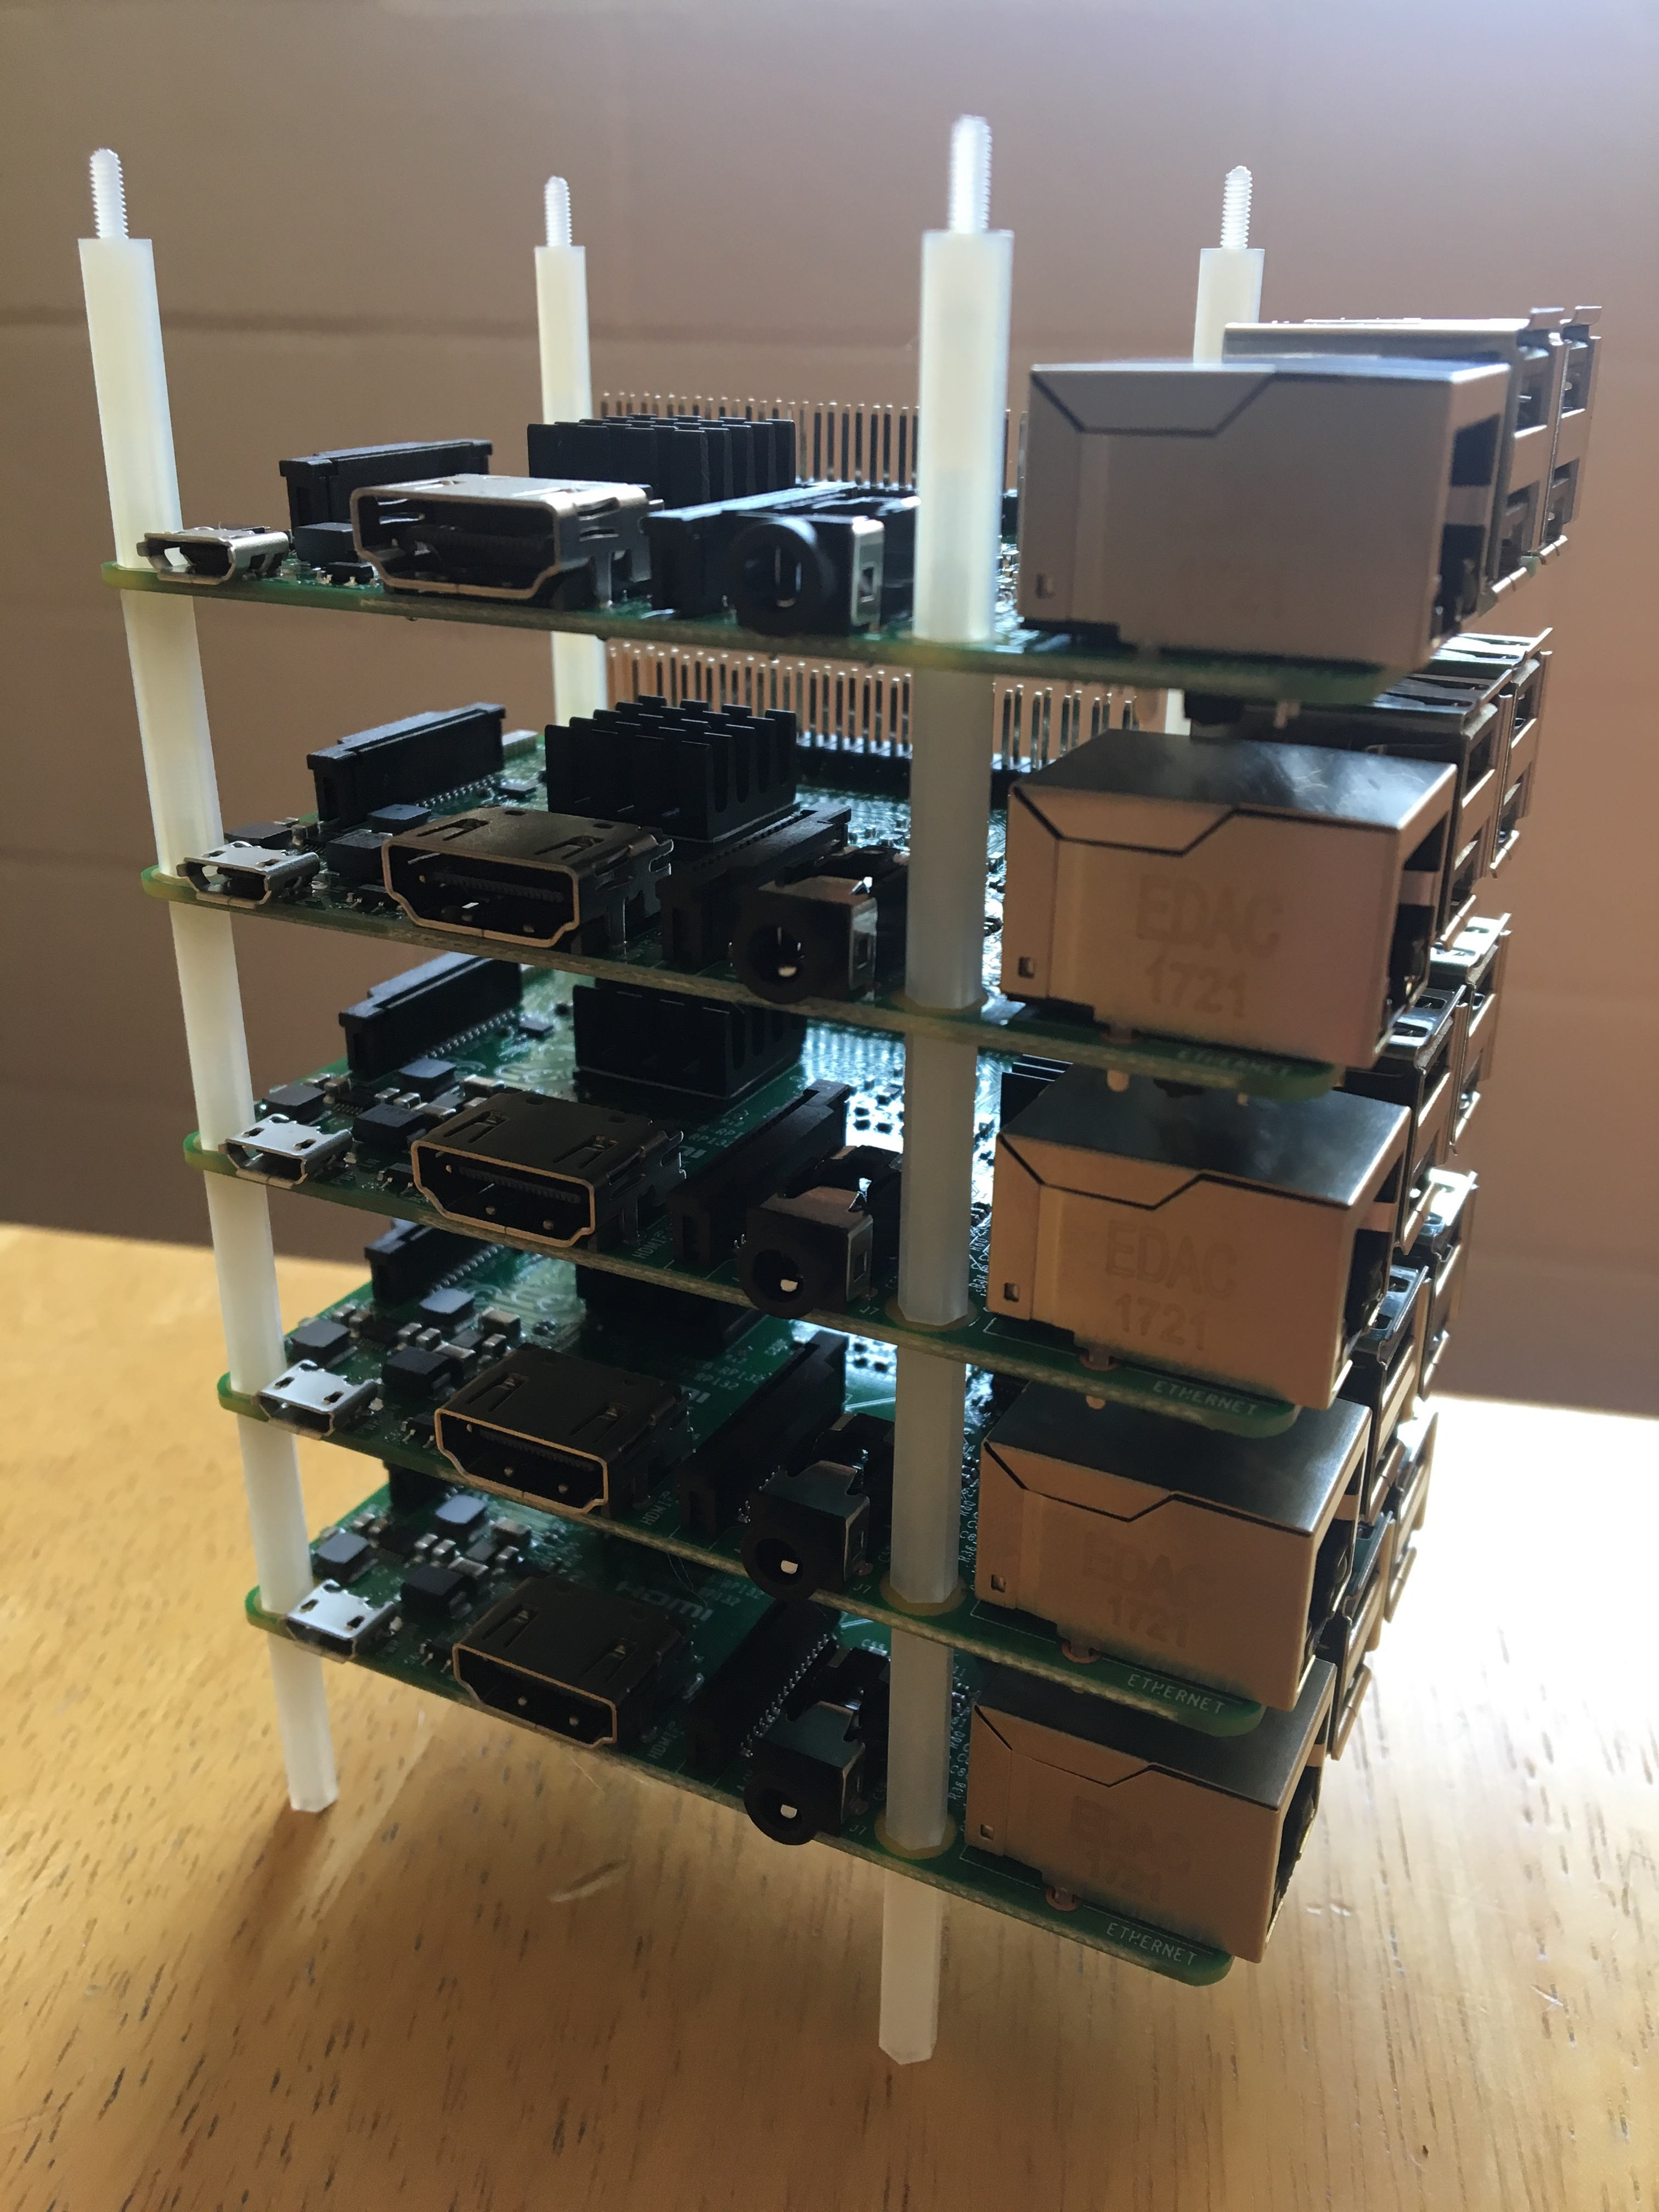
\includegraphics[width=\columnwidth]{images/pi-cluster-no-wires.jpg}

WRNING: line longer than 80 characters
       84: Each node of the cluster is then attached to the switch using the ethernet cables. 

WRNING: line longer than 80 characters
       101: Lee~\cite{hid-sp18-405-sentiment-pang2004asentimental}~\cite{hid-sp18-405-sentiment-pang2002thumbs}.

WRNING: line longer than 80 characters
       82: Each of the review is in a format of text file, and each of the single line in a 

WRNING: line longer than 80 characters
       81: the text files. Therefore, we just need to split the text strings with space to 

WRNING: line longer than 80 characters
       91: online~\cite{hid-sp18-405-hadoopstreaming-nltk}~\cite{hid-sp18-405-hadoopstreaming-corpus}

WRNING: line longer than 80 characters
       85:  one with higher probability. The final output will be a text file and each line is 

Warning 24 in content.tex line 173: Delete this space to maintain correct pagereferences.
        \label{f:data}  
       ^
Warning 26 in content.tex line 299: You ought to remove spaces in front of punctuation.
As illustrated in Equation~\ref{eq:nb} , Equation~\ref{eq:sm}, and   
                                      ^
Warning 24 in content.tex line 352: Delete this space to maintain correct pagereferences.
        \label{f:algoresult}  
       ^
Warning 39 in content.tex line 358: Double space found.
        ~\cite{hid-sp18-405-sentiment-pang2002thumbs}}\label{f:pang-result}  
       ^
\end{verbatim}
\end{tiny}
